\documentclass[11pt]{article}
\usepackage[margin=1in]{geometry}
\usepackage[T1]{fontenc}
\usepackage[utf8]{inputenc}
\usepackage{lmodern}
\usepackage{booktabs}
\usepackage{array}
\usepackage{colortbl}
\usepackage{longtable}
\usepackage{tabularx}
\newcommand{\rowrule}{\arrayrulecolor{black!22}\midrule\arrayrulecolor{black}}
\renewcommand{\arraystretch}{1.18}
\usepackage{enumitem}
\usepackage{hyperref}
\usepackage{xcolor}
\usepackage{graphicx}
\usepackage{amsmath}
\hypersetup{colorlinks=true,linkcolor=blue!50!black,urlcolor=blue!50!black,breaklinks=true}
\setlist{nosep}
\setlength{\parskip}{4pt}
\setlength{\parindent}{0pt}
\definecolor{claude}{HTML}{7A55CC}
\definecolor{jev}{HTML}{2E9E63}
\definecolor{code}{HTML}{3A7BC0}

\title{DoomSat: playing Doom through a real mission stack, with a System One and a System Two}
\author{Kevin Horton, 22 September 2026\\\small Built with Claude Code, TypeSafe's \emph{jev}, NASA F\'{}, Yamcs, NASA Open MCT and ViZDoom.}
\date{}
\begin{document}
\maketitle

Repository: \url{https://github.com/Devonance/claude-jev-fprime-yamcs-openmct-doom}

\section*{1. The idea in one paragraph}
Doom is a stress test dressed up as a toy. It is interactive (uplink latency shows up as a character that turns late), high rate (a 320x240 frame every 100 ms has to be fragmented, framed, sent, deframed and reassembled), and self-validating (a dropped frame or a mis-decoded telemetry value is obvious to anyone watching). So we put the game behind a real flight computer and played it from the ground through a real mission control system: the game is a \textbf{payload} behind an \textbf{F\'{} v4.3} deployment, telemetry and image products go down as \textbf{CCSDS} frames into \textbf{Yamcs 5.12}, whose mission database is the \textbf{XTCE} generated from the F\'{} dictionary, and the ground side plays by uplinking F\'{} commands. The player is not a person: TypeSafe's \textbf{jev} answers the moment-to-moment questions (a System One, half a second per decision), and \textbf{Claude Sonnet 5} reads an after-action report when an episode ends and rewrites the questions jev plays with (a System Two). Code owns the loop. Nobody reads the level file; the character has to find the exit the way a person would.

\begin{center}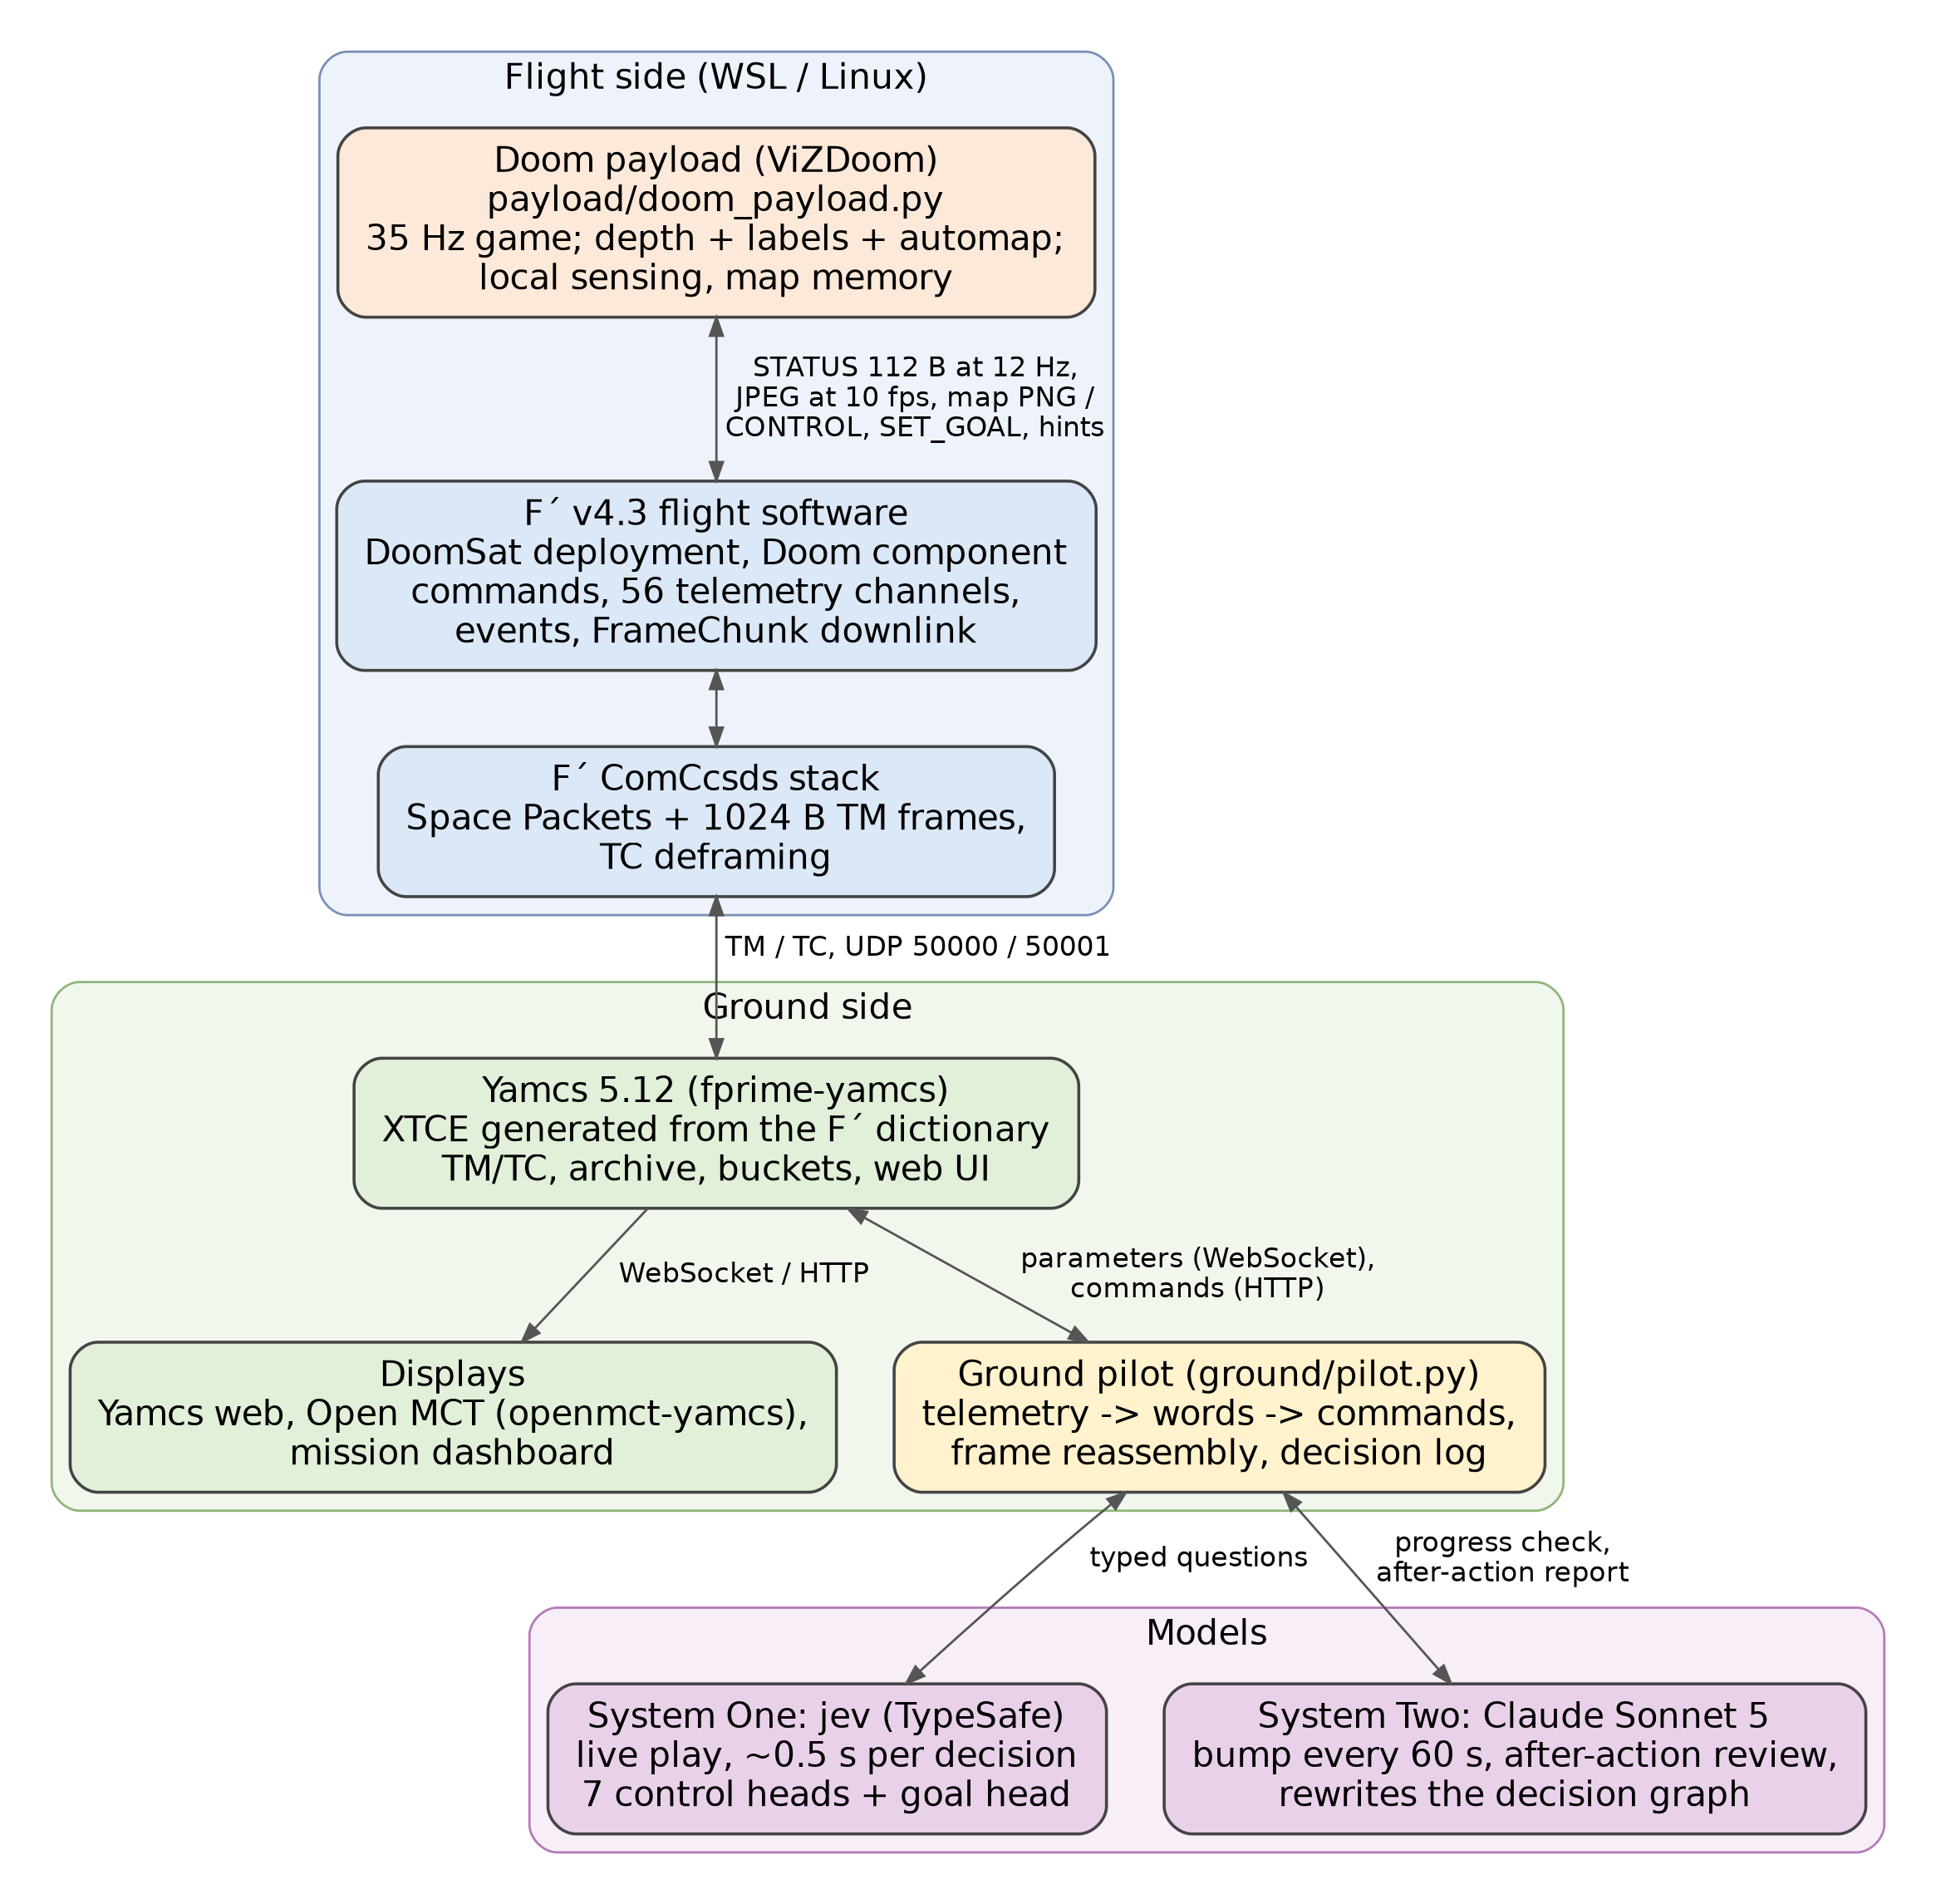
\includegraphics[width=\textwidth]{diagrams/architecture.png}\end{center}
\section*{2. Why two models and not one}
A large language model in a 35 Hz control loop is the wrong tool: 5 to 10 seconds per reply, and a reply that reasons about the whole situation when the situation only asks "turn left or right?". jev is the opposite: it answers a handful of typed multiple-choice questions in one forward pass in about 400 ms, and it gives a confidence per answer. That is the shape of a reflex. What it cannot do is notice, over many decisions, that a question is badly worded or a threshold is wrong. That is the shape of a review, and it is what the slow model is for. The split is therefore by \emph{timescale}, not by importance: jev plays every tick; Sonnet is consulted only between episodes, with a two-kilobyte report and the current graph, and returns a revised graph that code validates before the next episode uses it. Nothing slower than jev sits in the live loop.

This is the same pattern as the earlier Jezero rover demo (jev drives, Claude plans), moved onto a flight and ground stack and given a harder honesty rule.

\section*{3. What the system actually does}
\subsection*{3.1 The world}
The game is shareware Doom, level E1M1 onward, run by ViZDoom 1.3 at 35 Hz inside WSL. Finishing a level does not end the run: the payload advances to the next map and carries the weapons and ammunition over, as the game does (keys stay behind). Dying restarts the same level; the map the navigator built is kept, as a person's memory would be. Freedoom is the fallback when the shareware IWAD is not wanted.

\subsection*{3.2 What the player side may see}
The rule: jev and code go in blind, like a person who knows how to play Doom but has never seen this level. The level file is never read by the payload or the models. What replaces the person's eyes:

\begin{center}\small
\begin{tabular}{p{0.18\textwidth} p{0.34\textwidth} p{0.42\textwidth}}
\toprule
\textbf{Sense} & \textbf{What it stands in for} & \textbf{Source} \\
\midrule
Depth buffer (range camera) & where the walls are & ViZDoom depth buffer, calibrated: 7.16 map units per step, perpendicular distance \\ \rowrule
Object labels & recognising monsters, pickups, keys, barrels & ViZDoom labels buffer, only things in view \\ \rowrule
In-game automap, seen lines only & the map a player sees when pressing Tab & ZDoom automap in \texttt{NORMAL} mode: only lines the player has looked at, in the engine's default categories (wall, floor step, ceiling change = door, locked door in the colour of its key, exit line) \\ \rowrule
HUD variables & health, armor, ammo, position, heading & ViZDoom game variables \\
\bottomrule
\end{tabular}
\end{center}
Only the automap's colours are changed, so that code can read the categories off the pixels; no category is added and no unseen line is drawn. Not used: the automap's whole-map or show-objects modes, the "show trigger lines" option, sector or line geometry from the game state, monster counts, item lists, cheats. A WAD statistics script exists for the developer (choosing which levels to demo, checking results) and is never imported by the payload.

\subsection*{3.3 The onboard navigator}
The payload stamps the automap into a world raster (4 map units per pixel), sweeps free floor with the range camera, and plans on a 32-unit grid with a Dijkstra search whose edge costs come from the line categories: walls block, floor steps cost a little, doors cost more and get a Use press when reached, locked doors need the key of their colour, exit lines are destinations. Targets in priority order: an exit line it has seen, a key it has seen, the ground's goal item or enemy, the nearest unexplored frontier, and, when nothing is left, walls to try with Use (the exit switch is a wall until pressed). Things the automap does not draw, such as barred windows, fake doors and barrels, are learned: barrels and pillars from their labels, everything else by pushing against it once, after which that spot is a barrier for the rest of the level.

The navigator hands the ground a route bearing, a route length, clearances in the four directions (camera ahead, map to the sides and behind), what it is doing (exploring, at a door, fetching a key, hunting for a switch, heading for the exit) and what it is heading for.

\subsection*{3.4 The flight software and the link}
The F\'{} deployment is a fprime-bootstrap project with one custom component, \texttt{DoomMission::Doom}, on a 20 Hz rate group. It is a TCP client to the payload: a 76-byte status record twelve times a second becomes 44 telemetry channels, and each JPEG frame is split into 960-byte \texttt{FrameChunk} records that go straight into the com queue as telemetry packets (bypassing the channel sampler, which would drop most of them). Five commands go the other way: \texttt{CONTROL} (move, strafe, turn in degrees, fire, use, weapon), \texttt{SET\_GOAL}, \texttt{RESET\_GAME}, \texttt{FRAME\_RATE}, \texttt{EXPLORE\_HINT}. Events mark episodes, levels, keys, goals and dropped frames.

Downlink is the stock F\'{} \texttt{ComCcsds} stack: Space Packets (APID 1 telemetry, 2 events, 3 files) in fixed 1024-byte TM frames over UDP. The \texttt{fprime-yamcs} launcher generates the XTCE from the F\'{} JSON dictionary (148 parameters, 54 commands), starts Yamcs with it and bridges the frames. Yamcs decodes, archives and serves the parameters over its WebSocket and HTTP APIs, which is where the ground pilot, Open MCT and the dashboard read them.

\subsection*{3.5 The ground pilot and jev's decision graph}
\texttt{ground/pilot.py} subscribes to the Doom channels, reassembles frames, and every \textasciitilde{}0.5 s turns the numbers into words and asks jev. jev never sees a number: a route bearing of 37$^\circ$ is "left"; a clearance of 60 units is "tight"; a nearest enemy at 120 units is "close". The questions are the \emph{heads} of the graph, each a typed choice with criteria, and code decides which options are on the menu (Backward only when the space behind is known clear, strafes only when a side is clear, Use only when something is at arm's length):

\begin{center}\small
\begin{tabular}{p{0.18\textwidth} p{0.34\textwidth} p{0.42\textwidth}}
\toprule
\textbf{Head} & \textbf{Options} & \textbf{Decides} \\
\midrule
steer & Follow route / Left / Right / Back / Turn around & which way now, from the four clearances, when the route's way is blocked or the character is stuck \\ \rowrule
dodge & Carry on / Dodge left / right / back & evasion from a close enemy \\ \rowrule
move & Forward / Hold / Backward & advance \\ \rowrule
turn & Hard left ... Hard right / Turn around & put the aim (route waypoint or enemy) in the crosshair \\ \rowrule
fire & Fire / Hold fire & only with a living enemy in the crosshair and ammunition \\ \rowrule
weapon & Keep / Pistol / Shotgun & ammunition scarcity \\ \rowrule
use & Use / Wait & doors, switches, walls at arm's length \\ \rowrule
goal (every 4th tick) & Kill enemies / Restore health / Stock ammo / Add armor / Explore / Scout / Upgrade weapon & what the navigator should head for \\
\bottomrule
\end{tabular}
\end{center}
The answers map onto one \texttt{CONTROL} command. The steer head is the one that keeps the character from walking into the same wall twice: the onboard map is optimistic about things it cannot see, and when the eyes disagree with the route it is jev, not code, that picks the way out; the payload then remembers the dead end.

Turning is an onboard setpoint (the command says "turn 60 degrees", the payload executes it over ten tics), because a held turn rate with a half-second decision loop over-rotates. The pilot compensates bearings for the part of a commanded turn the heading does not show yet, and only that part.

\subsection*{3.6 System Two: the after-action review}
When an episode ends (death, level finished, run end) code writes a report of about two kilobytes: outcome, level, duration, decisions, health trace, damage taken with no enemy in view, cells explored, distance walked, stuck ticks, turn-direction flips, longest hold streak, per-head answer distributions with mean confidence, the navigator modes used and the last eight decisions in words. Sonnet gets the report and the current graph and returns a revised graph through a JSON-schema call: wording, criteria, thresholds (what counts as blocked, tight, close, critical), the turn sizes, how often the goal is re-asked, the standing order. Code validates the reply (fixed option names, known placeholders, numeric ranges), stores it as \texttt{graph\_v<N>.json} with the rationale in a changelog, and the next episode is played with it. The Claude CLI is run with non-essential model calls disabled, so the review is one Sonnet call and nothing else.

\subsection*{3.7 Displays}
Three views of the same Yamcs instance: the Yamcs web UI (parameters, command history, events, archive), Open MCT through the \texttt{openmct-yamcs} plugin (plots and the image product), and a one-page mission dashboard written for the recording, which shows the reassembled frame, the telemetry, jev's latest answers with the request latency, Sonnet's latest rationale, F\'{} events, the command archive and the map the navigator built.

\begin{center}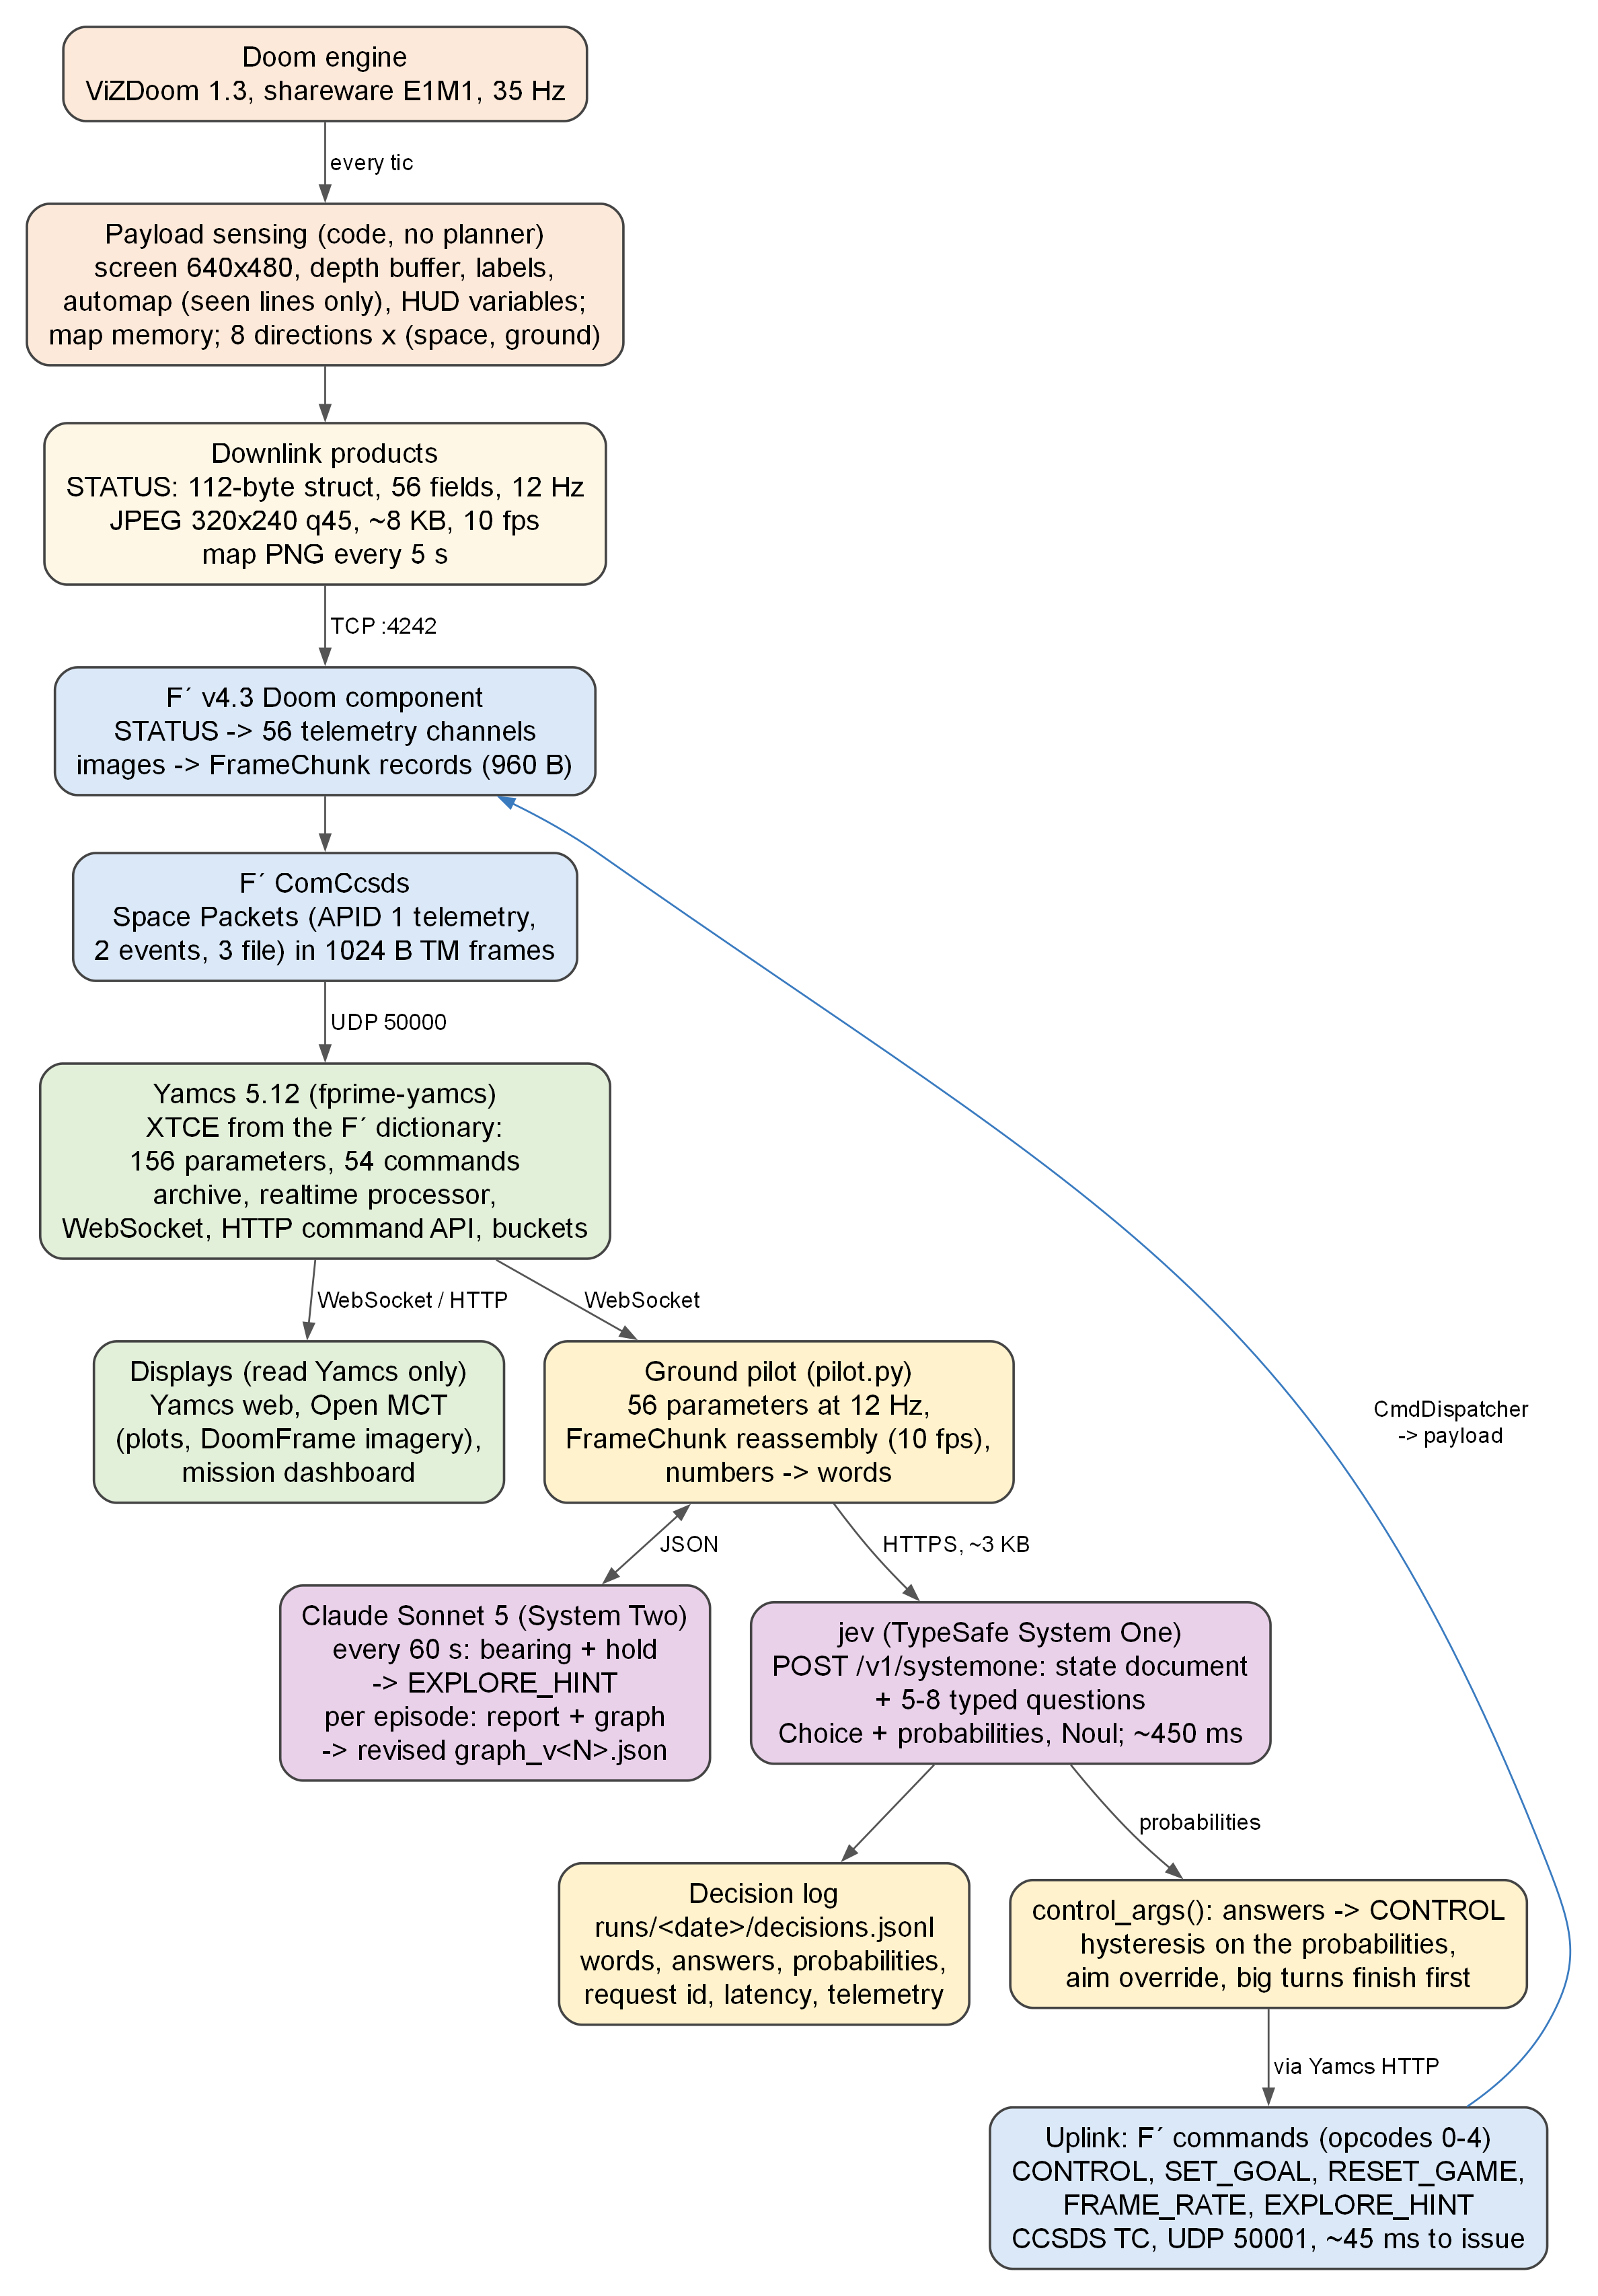
\includegraphics[width=\textwidth]{diagrams/dataflow.png}\end{center}
\section*{4. What each engine is trusted with, and why}
\begin{center}\small
\begin{tabular}{p{0.16\textwidth} p{0.14\textwidth} p{0.34\textwidth} p{0.28\textwidth}}
\toprule
\textbf{Layer} & \textbf{Runs} & \textbf{Trusted with} & \textbf{Not trusted with} \\
\midrule
Flight code (F\'{} + payload) & 35 Hz / 20 Hz & safety (uplink loss $\rightarrow$ hold still), the heading loop, the map, the route, door and switch attempts, level progression & any decision that a person would call judgement \\ \rowrule
jev (System One) & every \textasciitilde{}0.5 s & every control decision and the goal, from words & numbers, memory, the level layout \\ \rowrule
Claude Sonnet 5 (System Two) & between episodes & rewording and re-tuning the graph from evidence & anything live; it never touches the controls \\
\bottomrule
\end{tabular}
\end{center}
The reason the map lives onboard and not in jev's prompt is bandwidth and honesty at once: the automap is a picture, the route is a number, and jev should get the one word it needs ("the route goes to the left, space left is clear"), not a map to reason about in 400 ms.

\section*{5. Measuring instead of asserting}
Things that were measured rather than assumed, and what they changed:

\begin{itemize}
  \item \textbf{The depth buffer is perpendicular distance, 7.16 map units per step.} The first calibration (8.5, radial) put off-centre rays up to 25\% short; every wall the camera swept landed inside the room. A rotation test settled it: a wall point keeps its depth times the cosine of its bearing as the view turns.
  \item \textbf{Depth 0 is the sky.} Treating it as "very close" produced phantom walls in every outdoor view.
  \item \textbf{The crosshair is drawn into the depth buffer} (depth 0 at the centre pixel), and the automap crosshair and player arrow are drawn over the map lines beneath them. The arrow rotates with the heading, so the wall pixels under it flickered between stamps and the route flip-flopped between two equal paths every replan. The fix keeps the previously mapped pixels under the arrow.
  \item \textbf{A Yamcs bucket holds 1000 objects.} Frame uploads failed with HTTP 500 once yesterday's products filled it; the products now go into a ring of 20 names.
  \item \textbf{jev's latency} through the whole chain: \textasciitilde{}450 ms median per decision (eight heads), command issue through Yamcs \textasciitilde{}45 ms, telemetry at 12 Hz, frames at 10 fps with about one incomplete frame per thousand.
  \item \textbf{A turn commanded and a turn observed are different things.} Subtracting the whole commanded turn from the next bearing, after the telemetry already showed the turn done, made jev turn straight back: hard left, hard right, hard left. Subtracting only the part not yet observed removed the oscillation.
\end{itemize}
\section*{6. What we did today, in order}
\begin{enumerate}
  \item Started from the Freedoom MAP01 setup with a range-camera-only map. It stalled at every door, because a depth camera cannot tell a closed door from a wall.
  \item Looked at what other Doom agents do. The System One demo this graph descends from reads the WAD for the exit and the collision grid; the GPT-4/5 work used screenshots plus a written walkthrough. Neither is blind.
  \item Chose the in-game automap in seen-lines mode as the honest map, confirmed in the engine source that its categories are the defaults a person sees, calibrated its scale (\texttt{viz\_am\_scale}) and colours against the palette.
  \item Switched to shareware Doom E1M1 onward (the standard demo level), added level progression with weapon carry-over, keys, locked doors, exit lines, switch hunting; added the new telemetry and events to the F\'{} component and rebuilt.
  \item Found, one at a time, the sensing mistakes listed in section 5, with code-only self-play harnesses that run the payload in-process at 4x real time.
  \item Put jev back in command and watched it fail the way a person would not: walking into the same fake door. Added the steer head so that jev chooses the way out from the four clearances, and fixed the turn compensation.
  \item Built the dashboard, the diagrams and this report.
\end{enumerate}
\section*{7. Using the pixels: letting jev classify what it sees}
The one thing the automap cannot give is what a wall \emph{is}: a plain wall, a door, a switch, an exit sign. A person reads the texture. jev cannot take an image, but it takes numbers and words quickly, so the honest next step is to turn the pixels of a wall segment into a few numbers and ask jev what it is:

\begin{itemize}
  \item Code already knows, from the depth buffer, which screen columns belong to the surface at arm's length and how far it is. Take that patch of the screen (say 40x60 pixels at the crosshair).
  \item Reduce it to a short vector a person could have written down: dominant colours (a switch has a small bright panel on a dull background; an exit sign is red with white; a door is a tall uniform slab), edge density (switches and signs are busy, walls are not), vertical symmetry, whether the patch repeats horizontally (a wall texture tiles, a door does not), height of the surface from the depth buffer (doors reach the ceiling, switch panels do not).
  \item Ask jev one typed question with those values in words: "The surface at arm's length is 64 units wide, reaches the ceiling, mostly grey with a small bright red-and-white rectangle in the middle, busy edges, does not tile. What is it?" with options wall / door / switch / exit sign / monster / pickup, and take the confidence.
  \item Code acts on the answer the way it now acts on the map categories: door $\rightarrow$ Use; switch $\rightarrow$ Use and remember; exit sign $\rightarrow$ destination; monster $\rightarrow$ combat heads.
\end{itemize}
This keeps the division of labour: code measures, jev judges, and the judgement is one 400 ms call per new surface, not one per tick. It would replace both the "walls to try" fallback and most of the reliance on the automap's door colouring, and it is the same trick that made the Jezero rover's science stops work: reduce the picture to a sentence, then ask the fast model.

\section*{8. Results}
See the run table in the README's status section and \texttt{python tools/run\_report.py} for the current run. The figures in the table below are from the runs of 22 September 2026 (shareware E1M1, jev live, Sonnet after-action).

\begin{center}\small
\begin{tabular}{p{0.13\textwidth} p{0.13\textwidth} p{0.13\textwidth} p{0.13\textwidth} p{0.13\textwidth} p{0.13\textwidth} p{0.13\textwidth}}
\toprule
\textbf{Run} & \textbf{jev decisions} & \textbf{Explored cells} & \textbf{Distance walked} & \textbf{Stuck ticks} & \textbf{Levels finished} & \textbf{Notes} \\
\midrule
1, no steer head & 687 & 121 & 27k units & 60 & 0 & walked into the fake door repeatedly; turns alternated hard left/right \\ \rowrule
2, steer head & 202 & 147 & 7.3k units & 0 & 0 & jev chose Left/Right/Back/Turn around in 52 of 202 decisions; turns still alternated \\ \rowrule
3, steer head + turn compensation fix & see README &  &  &  &  &  \\
\bottomrule
\end{tabular}
\end{center}
\section*{9. Honest limits}
\begin{itemize}
  \item The exit of E1M1 was not reached in the runs recorded here; the character explores the level without getting stuck but has not yet walked into the exit room. The next levers are the ones in section 7 and letting the after-action reviews run for more episodes.
  \item The automap's door and exit categories are the engine's defaults, but they are still a shortcut compared to reading textures; section 7 is the honest replacement.
  \item Open MCT loads and connects to Yamcs, but headless Chrome would not paint it for the screenshots; the dashboard is what the recording shows.
  \item The onboard navigator is more code than the brief wanted. Every piece of it exists because a sensing assumption turned out to be wrong; the list in section 5 is the honest account of that.
\end{itemize}
\section*{10. Sources}
\begin{itemize}
  \item NASA F\'{} v4.3.0: \url{https://github.com/nasa/fprime}
  \item fprime-yamcs and fprime-xtce: \url{https://github.com/fprime-community/fprime-yamcs,} \url{https://github.com/FarkasJoseph/fprime-xtce/tree/feature/binary-annotation-combined}
  \item Yamcs 5.12.8: \url{https://github.com/yamcs/yamcs}
  \item NASA Open MCT and the openmct-yamcs plugin: \url{https://github.com/nasa/openmct,} \url{https://github.com/akhenry/openmct-yamcs}
  \item TypeSafe jev: \url{https://docs.typesafe.ai/introduction,} \url{https://docs.typesafe.ai/sdk/python/api}
  \item Claude Sonnet 5 through Claude Code: \url{https://code.claude.com/docs}
  \item ViZDoom 1.3.0: \url{https://vizdoom.farama.org,} \url{https://github.com/Farama-Foundation/ViZDoom}
  \item Shareware Doom IWAD (Debian \texttt{doom-wad-shareware}), Freedoom: \url{https://freedoom.github.io}
  \item The System One demo: \url{https://github.com/sgoedecke/system-one}
  \item Prior LLM-plays-Doom work: \url{https://adriandewynter.substack.com/p/will-gpt-4-and-5-run-doom}
\end{itemize}
\end{document}